\chapter{Santa Claus}\label{chapter: SC}
% \\ {\small Last changes: \today}

\section{Introduction}

Formally, the \emph{Santa Claus} problem takes as input a set $M$ of children, a set $J$ of gifts,
and values $p_{ij} \in \{ 0,p_j\}$ for all $i \in M$ and $j \in J$. In other words, a child is
only interested in a particular subset of the gifts, but then its value only depends on the
gift itself. The goal is to find an assignment $\sigma : J \to M$ of gifts to children so that
$
  \min_{i \in M} \sum_{j \in \sigma^{-1}(i)} p_{ij}
$
is maximized.

The first major progress on this problem is due to Bansal and Sviridenko~\cite{SantaClaus-BansalSviridenko-STOC2006}, who showed a $O(\log \log n / \log \log \log n)$-approximation based on rounding a \emph{configuration LP}. The authors of \cite{SantaClaus-BansalSviridenko-STOC2006} also realized that in order to obtain a $O(1)$-approximation, it suffices to answer 
a purely combinatorial problem: show that
in a uniform bipartite hypergraph with equal degrees on all sides, there is a left-perfect matching that selects a constant fraction of nodes from original edges.
This question was affirmatively answered by Feige~\cite{ConstantIntegralityGapSantaClaus-Feige-SODA2008} who proved a large unspecified constant using the Lov{\'a}sz Local Lemma repeatedly.
Then Asadpour, Feige and Saberi~\cite{SantaClaus-AsadpourFeigeSaberi-APPROX2008} showed that
one can answer the question of \cite{SantaClaus-BansalSviridenko-STOC2006} by using a beautiful
theorem on hypergraph matchings due to Haxell~\cite{HypergraphMatchingsHaxell95}; 
their bound\footnote{The conference version \cite{SantaClaus-AsadpourFeigeSaberi-APPROX2008} provides a factor of 5, and it was improved to 4 in the journal version~\cite{SantaClaus-AsadpourFeigeSaberi-Journal-TALG2012}.} of 4 has been slightly improved to 3.84 by Jansen and Rohwedder~\cite{ConfigurationLP-for-SantaClaus-has-gap-atmost3.84-Arxiv2018} and then to 3.808 by Cheng and Mao~\cite{CM19}.
%in fact their bound of 4 on the integrality gap
%of the configuration LP for Santa Claus has not been improved. 
Recently, Jansen and Rohwedder~\cite{CompactLPforAllocationProblems-JansenRohwedder-SOSA18} also showed (still non-constructively) that it suffices to compare to a linear program with as few as $O(n^3)$ many variables and constraints, in contrast to the exponential size configuration LP.

A \emph{hypergraph} $\pazocal{H} = (X \dot{\cup} W,\pazocal{E})$ is called \emph{bipartite}
if $|e \cap X| = 1$ for all hyperedges $e \in \pazocal{E}$. A \emph{(left-) perfect matching} is a set of hyperedges $F \subseteq \pazocal{E}$ that are disjoint but cover each node in $X$. In general, finding perfect matchings in even bipartite hypergraphs is 
$\mathbf{NP}$-hard, but there is an intriguing sufficient condition: 
\begin{theorem}[Haxell~\cite{HypergraphMatchingsHaxell95}]
Let $\pazocal{H} = (X \dot{\cup} W,\pazocal{E})$ be a bipartite hypergraph with $|e| \leq r$ for all $e \in \pazocal{E}$. Then either $\pazocal{H}$
contains a left-perfect matching or there is a subset $C \subseteq X$ and a subset $U \subseteq W$
so that all hyperedges incident to $C$ intersect $U$ and $|U| \leq (2r-3) \cdot (|C|-1)$.
\end{theorem}
It is instructive to consider a ``standard'' bipartite graph with $r=2$.
In this case, if there is no perfect matching, then there is a set $C \subseteq X$ with at most 
$|C|-1$ many neighbors --- so Haxell's condition generalizes \emph{Hall's Theorem}. Unlike Hall's Theorem, 
Haxell's proof is non-constructive and based on a possibly exponential time augmentation argument.
Only very recently and with a lot of care, Annamalai~\cite{FindingPerfectMatchingsInHypergraphs-Annamalai-SODA16} managed to make the argument polynomial. This was accomplished by introducing some slack into the condition and assuming the parameter $r$ is a constant. Preceding \cite{FindingPerfectMatchingsInHypergraphs-Annamalai-SODA16}, 
Annamalai, Kalaitzis and Svensson~\cite{AlgoForSantaClaus-AnnamalaiKalaitzisSvenssonSODA15}
gave a non-trivially modified version of Haxell's argument for Santa Claus, which runs in polynomial time
and gives a $12.33$-approximation\footnote{To be precise they obtain a $(6+2\sqrt{10}+\varepsilon)$-approximation in time $n^{O(\frac{1}{\varepsilon^2}\log(\frac{1}{\varepsilon}))}$.}.
Recently, Cheng and Mao altered their algorithm to improve the approximation to 
$6 + \varepsilon$, for any constant $\varepsilon >0$~\cite{ChengM18}.
Our algorithm will also borrow a lot from \cite{AlgoForSantaClaus-AnnamalaiKalaitzisSvenssonSODA15}. 
However, through a much cleaner argument
we obtain a result that works in a more general matroid setting
and implies a better approximation of $4+\varepsilon$ for Santa Claus.


It should not go without mention that the version of the Santa Claus problem with arbitrary 
$p_{ij}$ has also been studied before under the name \emph{Max-Min Fair Allocation}. Interestingly, the integrality gap of the 
configuration LP is at least $\Omega(\sqrt{n})$~\cite{SantaClaus-BansalSviridenko-STOC2006}. 
Still, Chakrabarty, Chuzhoy and Khanna~\cite{MaxMinFairAllocation-ChakrabartyChuzhoyKhannaFOCS09}
found a (rather complicated) $O(\log^{10}(n))$-approximation algorithm in  $n^{O(\log n)}$ time\footnote{The
factor is $n^{\varepsilon}$ if only polynomial time is allowed, where $\varepsilon > 0$ is arbitrary but fixed.}.

Santa Claus has a very well studied ``dual'' minmax problem. 
Usually it is phrased as \emph{Makespan Scheduling} with \emph{machines} $i \in M$ 
and \emph{jobs} $j \in J$. Then we have a running time $p_{ij}$ of job $j$ on machine $i$, and the goal 
is to assign jobs to machines so that the maximum load of any machine is minimized.
In this general setting, the seminal algorithm of Lenstra, Shmoys and Tardos~\cite{SchedulingUnrelatedParallelMachines-LenstraShmoysTardos-FOCS87} gives a 2-approximation --- with no
further improvement since then. In fact, a $(\frac{3}{2}-\varepsilon)$-approximation is $\mathbf{NP}$-hard~\cite{SchedulingUnrelatedParallelMachines-LenstraShmoysTardos-FOCS87},
and the configuration LP has an integrality gap of 2~\cite{LowerBoundOnGapOfConfigurationLP-VerschaeWiese-ESA11}. In the restricted assignment setting
with $p_{ij} \in \{ p_j,\infty\}$, the breakthrough of Svensson~\cite{MakespanScheduling-Svensson-STOC11} provides a non-constructive $1.942$-bound on the integrality gap of the
configuration LP using a custom-tailored Haxell-type search method.
Recently, this was improved by Jansen and Rohwedder~\cite{ConfigurationLPforRestrictedAssignment-JansenRohwedderSODA17} to $1.834$. In an even more restricted variant called \emph{Graph Balancing}, each job is admissable on exactly 2 machines. In this setting Ebenlendr, Krc{\'{a}}l and Sgall~\cite{GraphBalancingEbenlendrKS-SODA08}
gave a 1.75-approximation based on an LP-rounding approach, which has again been improved by Jansen
and Rohwedder~\cite{GraphBalancing1.749-apx-with-local-search-Arxiv2018} to 1.749 using a local search argument.

%{\bf MISSING: CONTINUE DISCUSSING MAKESPAN SCHEDULING!}

%could also be called more technically, \emph{(Restricted) Max Min Fair Allocation}
%See \cite{AlgoForSantaClaus-AnnamalaiKalaitzisSvenssonSODA15}.

\subsection{Our contributions}\label{sec: contributions}

Let $\pazocal{M} = (X,\pazocal{I})$ be a \emph{matroid} with \emph{groundset} $X$ and 
a family of \emph{independent sets} $\pazocal{I} \subseteq 2^X$. Recall that 
a matroid is characterized by three properties: 
\begin{enumerate*}
\item[(i)] \emph{Non-emptyness}: $\emptyset \in \pazocal{I}$; 
\item[(ii)] \emph{Monotonicity}: For $Y \in \pazocal{I}$ and $Z \subseteq Y$ one has $Z \in \pazocal{I}$; 
\item[(iii)] \emph{Exchange property}: For all $Y,Z \in \pazocal{I}$ with $|Y| < |Z|$ there is an element $z \in Z \setminus Y$ so that $Y \cup \{ z\} \in \pazocal{I}$.
\end{enumerate*}
The \emph{bases} $\pazocal{B}(\pazocal{M})$ of the matroid are all inclusion-wise maximal independent sets. The cardinalities of 
all bases are identical, with size denoted as $\textrm{rank}(\pazocal{M})$.
The convex hull of all bases is called the \emph{base polytope}, that is $P_{\pazocal{B}(\pazocal{M})} := \textrm{conv}\{ \chi(S) \in \{0,1\}^X \mid S\textrm{ is basis}\}$,
where $\chi(S)$ is the \emph{characteristic vector} of $S$.


Now consider a bipartite graph $G = (X \dot{\cup} W,E)$ with the ground set $X$ on one side and
a set of \emph{resources} $W$ on the other side; each resource  $w \in W$ has
a \emph{size}  $p_w \geq 0$. 
In a problem that we call \emph{Matroid Max-Min Allocation}, 
the goal is to find a basis $S \in \pazocal{B}(\pazocal{M})$ and an 
assignment $\sigma : W \to S$ with $(\sigma(w),w) \in E$ so that $\min_{i \in S} \sum_{w \in \sigma^{-1}(i)} p_w$ is maximized. 
To the best of our knowledge, this problem has not been studied before.
In particular if $T \geq 0$ is the target objective function value, then 
we can define a linear programming relaxation $Q(T)$ as the set of vectors $(x,y) \in \setR_{\geq 0}^X \times \setR_{\geq 0}^E$
satisfying the constraints
\begin{eqnarray*}
 x \in P_{\pazocal{B}(\pazocal{M})}; \quad 
 \sum_{w \in N(i)} p_wy_{iw} \geq T \cdot x_i \;  \forall i \in X; \quad  y(\delta(w)) \leq 1 \; \forall w \in W; \quad y_{iw} \leq x_i \; \forall (i,w) \in E.
\end{eqnarray*} 

Here, the decision variable $x_i$ expresses whether element $i$ should be part of the basis, and
$y_{iw}$ expresses whether resource $w$ should be assigned to element $i$. We abbreviate 
$N(i)$ as the neighborhood of $i$ and $y(\delta(w))$ is shorthand for $\sum_{i : (i,w) \in E} y_{iw}$.
Then our main technical result is: 
\begin{theorem} \label{thm:MainMatroidAlgorithm}
Suppose $Q(T) \neq \emptyset$. Then for any $\varepsilon>0$ one can find
 \[
   (x,y) \in Q \left (
    \left (\frac13 - \varepsilon \right ) \cdot T - \frac13 \cdot \max_{w \in W} p_w \right )
 \] 
with both $x$ and $y$ integral in time $n^{\Theta_{\varepsilon}(1)}$, where $n := |X| + |W|$.
This assumes that membership in the matroid can be tested in time polynomial in $n$. 
\end{theorem}
Previously this result was not even known with non-constructive methods. 
We see that Matroid Max-Min Allocation is a useful framework by applying it to the Santa Claus problem:
%\rem{T: We need to say something about whether or not we are
%aware of a multiplicative approximation factor for Matroid Max-Min Allocation. 
%Recall that testing whether the optimum is even positive can be done with matroid intersection.} Given the generality of matroids, we feel this is
%a fairly useful result for constructing approximation algorithms. T: DONE!

%However, using Theorem~\ref{thm:MainMatroidAlgorithmYIntegral} as a blackbox we can get:
\begin{theorem}
The Santa Claus problem admits a $(4+\varepsilon)$-approximation algorithm in time
$n^{\Theta_{\varepsilon}(1)}$. 
\end{theorem}

For a suitable threshold $0<\delta<1$, call a gift $j$ \emph{small} 
if $p_j \leq \delta \cdot OPT$ and \emph{large} otherwise. Then the family of sets of children that can get 
assigned large gifts forms a \emph{matchable set matroid}. We apply 
Theorem~\ref{thm:MainMatroidAlgorithm} to the \emph{co-matroid} of the matchable set matroid.
Then we obtain a basis $S := \{ i \in M \mid x_i=1\}$, 
which contains the children \emph{not} receiving a large gift. 
These children can receive small gifts of total value $( \frac{1}{3}- \frac{\delta}{3} -\varepsilon) \cdot OPT$. 
The remaining children receive a large gift with value at least $\delta \cdot OPT$.
Setting $\delta := \frac{1}{4}$ implies the claim. 
Note the approximation factor $4+\varepsilon$ will be with respect to a natural, 
compact linear program with $O(n^2)$ many variables and constraints. 
The smallest LP that was previously known to have a constant integrality gap was the $O(n^3)$-size LP of \cite{CompactLPforAllocationProblems-JansenRohwedder-SOSA18}.
%that we define later in Section~\ref{sec:SantaClausApplication}.


\section{An algorithm for Matroid Max-Min Allocation}

In this section we provide an algorithm that proves 
Theorem~\ref{thm:MainMatroidAlgorithm}. 

\subsection{Intuition for the algorithm}

We provide some insight by starting with an informal overview of our algorithm.
Let $G = (X \cup W,E)$ be the bipartite graph defined in Section~\ref{sec: contributions}.
If $U \subset W$ and $i \in X$ with $(i,j) \in E$ for all $j \in U$, 
we can consider the pair $(i,U)$ to be a hyperedge.
Then for $0<\nu <1$ and val$(\cdot)$ the function summing the value in a hyperedge's resources,
we say that $(i,U)$ is a \emph{$\nu$-edge} if it a hyperedge with
minimal (inclusion wise) resources such that val$(U) := \sum_{w \in U} p_w \geq \nu T$.
By $\pazocal{E}_{\nu T}$ we denote the set of $\nu$-edges.
% \[
%   \pazocal{E}_{\nu T}  = \{(i,S) \text{ a } \nu\text{-edge} \} \qquad E_A = \{(i,S) \text{ an } \alpha\text{-edge} \}
% \]
%  and and abbreviate hyperedges of size $t$ as 
% \[
%   \pazocal{E}_{t} := \{ e=(i,W') \mid  i \in X\textrm{ and }W' \subseteq \delta(i)\textrm{ with }|W'| = t\}.
% \]

Fix constants $0< \beta<\alpha<1$ and $0<\delta < 1$, to be chosen later.
The goal of the algorithm is to find a basis $S \in \pazocal{B}(\pazocal{M})$
and a hypergraph matching $M \subseteq \pazocal{E}_{\beta T}$ covering $S$. 
The algorithm is initialized with $S := \{i_0\}$, for any node $i_0 \in X$,
and $M := \emptyset$. 
We perform rank($\pazocal{M}$) many phases, 
where in each phase we find a larger matching,
and the set it covers in $X$ is independent with respect to the matroid.
In an intermediate phase, we begin with
$S \in \pazocal{I}$ and $M \subseteq \pazocal{E}_{\beta T}$
a hypergraph matching covering $S \setminus \{ i_0\}$ with one exposed node $i_0 \in X$. 
At the end of a phase, the algorithm produces an updated matching covering an independent set $S'$, with $|S'|=|S|$.
For $|S'| < \textrm{rank}(\pazocal{M})$, there exists $i_0' \in X \setminus S'$ such that $S' \cup \{i_0'\} \in \pazocal{I}$.
 Repeating this $\text{rank}(\pazocal{M})$ times, we end with a basis which is well-covered by $\beta$-edges. 
% \rem{S: Changed 2nd paragraph}

The algorithm generalizes the notion of an augmenting path used 
to find a maximum matchings in bipartite graphs to an \textit{augmenting tree}.
Though instead of swapping every other edge in an augmenting path, as is the case for a bipartite graph, 
the algorithm swaps sets of edges in the augmenting tree to find more space in the hypergraph.
During a phase, the edges are swapped in such a way that the underlying set in $X$ covered by the matching 
is always independent with respect to the matroid. The edges which are candidates for being
swapped into the matching are called \textit{adding edges} and denoted by $A$, while those 
which are candidates for being swapped out of the matching are called \textit{blocking edges} 
and denoted by $B$. 
It is helpful to discuss the nodes covered by adding and blocking edges in each part,
and so for hyperedges $H \subseteq \pazocal{E}_{\nu T}$ we define $H_X$ and $H_W$
as the nodes covered by $H$ in $X$ and $W$, respectively.
The algorithm gives some slack by allowing the adding edges to be slightly larger than the blocking edges.

The parameters $\alpha$ and $\beta $ determine the value of the adding and blocking edges, respectively,
so the adding edges are a subset of $\pazocal{E}_{\alpha T}$
while the blocking edges are a subset of $\pazocal{E}_{\beta T}$.
Set $\delta := \max_w p_w / T$, so that
all elements in the basis receive resources with value at most $\delta T $.
The following observations follow from minimality of the hyperedges: 
\begin{enumerate}
\item A $\nu$-edge has value less than $(\nu + \delta)T$. 
This implies that an add edge has value less than $ ( \alpha + \delta )T$ and a blocking edge has value less than $ (\beta + \delta) T$.
\item Every blocking edge has value at most $\beta \cdot T$ not covered by an add edge.
\end{enumerate}


To build the augmenting tree,
 the algorithm starts from the node in $S$ uncovered by $M$, $i_0$,
  and chooses an edge $e \in \pazocal{E}_{\alpha T}$ covering $i_0$ which is added to $A$.
If there is a large enough hyperedge $e' \in \pazocal{E}_{\beta T}$ such that $e' \subset e$ and $e'$ is disjoint from $M$,
then there is enough available resources that we simply update $M$ by adding $e'$ to it.
Otherwise, $e$ does not contain a set of resources with total value $\beta T$ free from $M$. 
The edges of $M$ intersecting $e$ are added to the set of blocking edges, $B$. 
Nodes in $C=\{i_0\} \cup B_X$ are called \textit{discovered} nodes,
 as they are the nodes covered by the hypermatching $M$ which appear in the augmenting tree. 

Continuing to build the augmenting tree in later iterations, 
the algorithm uses an \textit{Expansion Lemma} to find a large set of disjoint hyperedges, 
$H \subset \pazocal{E}_{\alpha T}$, that cover a subset which can be swapped into $S$ in place of some subset of 
$C$ while maintaining independence in the matroid. 
The set of hyperedges $H$ either $(i)$ intersects many edges of $M$ or 
$(ii)$ has a constant fraction of  edges which contain a hyperedge from $\pazocal{E}_{\beta T}$ that is disjoint from $M$. 


In the first case, a subset of $H$ which intersects $M$, denoted $A_{\ell+1}$, 
is added to $A$,
and the edges of $M$ intersecting $A_{\ell+1}$, denoted $B_{\ell+1}$, are added to $B$, 
for $\ell$ the index of the iteration. 
Note we naturally obtain \textit{layers} which partition the adding and blocking edges in our augmenting tree. 
The layers for the adding and blocking edges respectively are denoted as $A_{\ell}$ and $B_{\ell}$, with 
\[
A_{\leq \ell} := \bigcup\limits_{i=0}^{\ell} A_i \qquad \text{ and }  \qquad B_{\leq \ell}:=\bigcup\limits_{i=0}^{\ell}B_i.
\]
The layer indices are tracked because they are useful in proving the algorithm's runtime. 
In the second case, for the set of edges $H' \subset \pazocal{E}_{\alpha T}$ 
that have a hyperedge from $\pazocal{E}_{\beta T}$ disjoint from $M$, 
the algorithm finds a layer which has a large number of discovered nodes that can be swapped out for a subset of nodes which $H'$ covers. 

\subsection{A detailed procedure}
   
      
% In settings where $\delta \leq \frac14$, it is best to let $\delta$ remain unchosen and set 
Recall, we fixed $\delta = \max_{w \in W} p_w/T$. 
Then, we set
$\beta = \frac{1}{3}  - \frac{\delta}{3} -\varepsilon$ and $\alpha = \frac{1}{3} - \frac{\delta}{3} -\frac{\varepsilon}{2}$, for 
$0<\varepsilon < (1-\delta)/3$.
% If $\delta > \frac14$,
% it is best to cap $\delta$ at $\frac14$ so that $\beta = \frac{1}{4} -\varepsilon$ 
% and $\alpha = \frac{1}{4} -\frac{\varepsilon}{2}$, for $0<\varepsilon<\frac14$.
Here lies the subtle but crucial difference 
to previous work. In \cite{AlgoForSantaClaus-AnnamalaiKalaitzisSvenssonSODA15} the authors have
to use adding edges that are a large constant factor bigger than blocking edges. In our setup we can allow 
adding edges that are only marginally larger than the blocking edges.
 This results in an improved approximation factor of 
$4+\varepsilon$ for Santa Claus compared to the $12.33$ factor by \cite{AlgoForSantaClaus-AnnamalaiKalaitzisSvenssonSODA15}.

The algorithm is described in Figure~\ref{fig:Algorithm}. For later reference, 
 the constant from Lemma~\ref{lem:GreedyMatchingExpansionLemma} is 
 $\frac{1-2\alpha-\beta - \delta}{1+\delta} = \frac{2\varepsilon}{1+\delta}\geq  \varepsilon$, and 
the constant from Lemma~\ref{lem:SizeOfOverlapOfNewEdgesWithM} is 
$\frac{\alpha -\beta}{\delta + \alpha} = \frac{\varepsilon}{2(1+\delta)}  \geq \varepsilon/4$.
We use Lemma~\ref{lem:ConstantSizeSwap}, with constant
$c = \frac{1-2\alpha-\beta -\delta}{1+\delta} \cdot \frac{\alpha - \beta}{\delta+\alpha}$. 
Our bounds for constants do not use a specific choice of $\delta$, 
and instead they only use the fact that $0 < \delta <1$.
%In the algorithm, $\gamma>0$ is the constant from Lemma~\ref{lem:ConstantSizeSwap}.
% \rem{T: Removed a sentence here.}
%and $\gamma \geq \frac{1}{2\left (1+\frac{\log \left (\frac{2}{3 \varepsilon^2} \right)}{\log(1+3 \varepsilon^2)}\right)}$. 
%Note in the algorithm, the fraction of swappable nodes in a layer is at worst half that of Lemma~\ref{lem:SizeOfOverlapOfNewEdgesWithM}, as we might have to exclude our root node $i_0$ from being swapped. 
Both cases in the algorithm are visualized in Figure~\ref{fig:CaseIofTheAlgorithm} and
Figure~\ref{fig:CaseIIofTheAlgorithm}.


\begin{figure}
\hrule \vspace{2mm}
%\begin{algorithm}
\begin{algorithmic}
  {\small 
\State {\bf Input:} Node $i_0$ and set $S \in \pazocal{I}$ with $i_0 \in S$. Matching $M \subseteq \pazocal{E}_{\beta T}$ with $M_X = S \setminus \{i_0\}$.

\State Initialize: $A=A_0 = \emptyset$, $B=B_0 = \emptyset$, $C = \{i_0\}$, $\ell=0$.

\smallskip
\While{TRUE} %\While{While $i_0$ is unmatched by $M$}
\State Find disjoint $H \subseteq \pazocal{E}_{\alpha T}$
covering $D \subseteq (X \setminus S) \cup C$, s.t. 
$|D| \geq \varepsilon \cdot |C|$, $(S \setminus C) \cup D \in \pazocal{I}$, *and $H_W$ is disjoint from $A_W \cup B_W$.
\\ 
\\
\textit{//\;Build the next layer in the augmenting tree}
\If{$H$ intersects at least $ \frac{\varepsilon}{4} \cdot |H| \geq \frac{\varepsilon^2}{4} \cdot |C|$ many edges $M$ on $W$-side}
\State $ B \leftarrow B \cup B_{\ell+1}$, $B_{\ell+1} =\{e \in M : e \cap H \neq \emptyset\}$
\State \textit{//\;Find subset of $H$ to add to $A$}
\Indent
  \For{ $b \in B_{\ell +1}$}
  \State Choose one edge $h_b \in H$ such that $h_b \cap b \neq \emptyset$
  \State $A_{\ell +1} \leftarrow A_{\ell+1} \cup \{h_b\}$
  \EndFor
\EndIndent
\State $C \leftarrow B_X \cup \{ i_0\}$
\State $\ell \leftarrow \ell + 1$
\\
\\
\textit{// \; Swap sets and collapse layers}
\Else { $ H'=\{e \in H : \text{val}(e_W \setminus M_W) \geq \beta T \}$ has size at least $  \frac{\varepsilon}{4} \cdot |H|$} 
\State  For all $e \in H'$, choose one $e ' \subset e$ with $e' \in \pazocal{E}_{ \beta T}$ and $e'_W \cap M_W = \emptyset$.
 Replace $e$ for $e'$ in $H'$.
%If $|H'| \geq 2$ and $i_0 \in H'_X$ then delete edge covering $i_0$.
\State \textit{//\;Find a set to swap in, $\tilde{D}$, and a set to swap out, $\tilde{C}$}
\Indent 
  \State $D' \subseteq D$ are the nodes covered by $H'$
  \State $C' \subseteq C$ is such that $|C'|=|D'|$ and $S \setminus C' \cup D' \in \pazocal{I}$ %(and if possible $i_0 \notin C'$).
  \If {$i_0 \in C'$}
    \State Let $i_1 \in D'$ so that $S' := S \setminus \{ i_0\} \cup \{ i_1\} \in \pazocal{I}$ and let $e_1 \in H'$ be edge covering $i_1$.
    \State Return $M' := M \cup \{ e_1\}$ covering all of $S'$ and \textbf{terminate}.
  \EndIf 
%  \If {$i_0 \in C' \setminus D'$}
%  \State For $k_0 \in D'$ such that $(S \setminus C' \cup D') \cup \{k_0\} \setminus \{i_0\} \in \pazocal{I}$, remove $k_0$ from $D'$.
%  \State Remove the edge covering $k_0$ from $H'$.
%  \State Remove $i_0$ from $C'$. 
%  \EndIf
  \State Layer $\tilde{\ell} \leq \ell$ contains  $\tilde{C} \subset C' \cap (B_{\tilde{\ell}})_X$, with $|\tilde{C}| \geq \gamma|C'|$. **
  \State Let $\tilde{D} \subset D'$ be such that $|\tilde{C}| = |\tilde{D}|$ and $S' := S \setminus \tilde{C} \cup \tilde{D} \in \pazocal{I}$.
  \State $\tilde{M} \subset M$ covers $\tilde{C}$ and $\tilde{H} \subset H'$ covers $\tilde{D}$. 
\EndIndent

\State $M \leftarrow M \setminus \tilde{M} \cup \tilde{H}$, and $S \leftarrow S'$ 
\State $A \leftarrow A_{\leq \tilde{\ell}}$, $B \leftarrow B_{\leq \tilde{\ell}} \setminus \tilde{M}$, $C \leftarrow B_X \cup \{ i_0\}$
\State $\ell \leftarrow \tilde{\ell}$
\EndIf ***
\EndWhile

\smallskip }
\footnotesize{
* Possible by Lemma~\ref{lem:GreedyMatchingExpansionLemma} with $W' := A_W \cup B_W$. 

** By Lemma~\ref{lem:ConstantSizeSwap}, such a $\tilde{C}$ exists.

*** One of the conditionals occurs by Lemma~\ref{lem:SizeOfOverlapOfNewEdgesWithM}.}
\end{algorithmic}
\hrule
\caption{Main algorithm} \label{fig:Algorithm}
%\end{algorithm}
\end{figure}
% \rem{T: In the algorithm I changed the WHILE condition and added a termination condition.}
%\rem{T: In the algorithm, I changed the initialization $A_0 = \{ (i_0,\emptyset)$ to $A_{0} = \emptyset$. I believe/hope this is consistent with the algorithm. I saw this as necessary because we claim the invariant of $|A_{\leq \ell}| \leq |B_{\leq \ell}|$ which is false otherwise.}


\subsection{Correctness of the algorithm}
Here, we prove several lemmas used in the algorithm which implies Theorem~\ref{thm:MainMatroidAlgorithm}. 
We begin by building up to our \textit{Expansion Lemma}, Lemma~\ref{lem:GreedyMatchingExpansionLemma}. 
Our algorithm takes a fixed independent set, $S$, and swaps $C \subset S$ out of $S$ for a set of nodes $D$
in order to construct a new independent set of the same size.
This is possible by Lemma~\ref{lem:GreedyMatchingExpansionLemma}. 

Recall a variant of the so-called \emph{Exchange Lemma}.
 For independent sets $Y,Z \in \pazocal{I}$, let $H_{\pazocal{M}}(Y,Z)$ 
 denote the bipartite graph on parts $Y$ and $Z$ (if $Y \cap Z \neq \emptyset$, 
 then have one copy of the intersection on the left and one on the right).
For  $i \in Y \setminus Z$ and $j \in Z \setminus Y$ we insert an edge $(i,j)$ 
in $H_{\pazocal{M}}(Y,Z)$ if $Y \setminus \{ i\} \cup \{ j\} \in \pazocal{I}$. 
Otherwise, for $i \in Y \cap Z$, there is an edge between the left and right copies of $i$,
 and this is the only edge for both copies of $i$. 

\begin{lemma}[Exchange Lemma]\label{lem:ExchangeLemma}
For any matroid $\pazocal{M} = (X,\pazocal{I})$ and independent set $Y,Z \in \pazocal{I}$ with $|Y| \leq |Z|$,
the exchange graph $H_{\pazocal{M}}(Y,Z)$ contains a left perfect matching.
\end{lemma}



Next, we prove several lemmas about vectors in the base polytope with respect to sets containing swappable elements.
Lemma~\ref{lem:GreedyMatchingExpansionLemma} relies on a \textit{Swapping Lemma}, 
Lemma~\ref{lem:SumOverBasePolytopeGeneral}, for which the next lemma serves as a helper function.
\begin{lemma}[Weak Swapping Lemma] \label{lem:SumOverBasePolytope}
Let $\pazocal{M} = (X,\pazocal{I})$ be a matroid with an independent set $S \in \pazocal{I}$.
For $C \subseteq S$, define 
\[
    U := \{ i \in (X \setminus S) \cup C \mid (S \setminus C) \cup \{i\} \in \pazocal{I}\}.
\]
Then for any vector $x \in P_{\pazocal{B}(\pazocal{M})}$ in the base polytope one has $\sum_{i \in U} x_i \geq |C|$.
\end{lemma}
\begin{proof}
Note that in particular $C \subseteq U$. Moreover, an equivalent definition of $U$ is 
\[
    U = \{ i \in (X \setminus S) \cup C \mid \exists j \in C: (S \setminus \{j\}) \cup \{ i\} \in \pazocal{I}\}.
\]
Due to the integrality of the base polytope, there is a basis $B \in \pazocal{I}$ 
with $\sum_{i \in U} x_i \geq \sum_{i \in U} (\chi(B))_i = |U \cap B|$, 
where $\chi(B) \in \{ 0,1\}^X$ is the characteristic vector of $B$. 
As $S$ and $B$ are independent sets with $|S| \leq |B|$, 
from Lemma~\ref{lem:ExchangeLemma} there is a left-perfect matching in the exchange graph $H_{\pazocal{M}} (S,B)$. 
The neighborhood of $C$ in $H_{\pazocal{M}} (S,B)$ is  $U \cap B$.
As there is a left-perfect matching, $|B \cap U|$ is least $|C|$ and hence $\sum_{i \in U} x_i \geq |U \cap B| \geq |C|$.
% and hence $\sum_{i \in D} x_i \geq |B \cap D| \geq |C|$. 
\end{proof}

Next, we derive a more general form of the Swapping Lemma (which coincides
with the previous Lemma~\ref{lem:SumOverBasePolytope} if $D = \emptyset$): 
\begin{lemma}[Strong Swapping Lemma] \label{lem:SumOverBasePolytopeGeneral}
Let $\pazocal{M} = (X,\pazocal{I})$ be a matroid with an independent set $S \in \pazocal{I}$.
Let $C \subseteq S$ and $D \subseteq (X \setminus S) \cup C$ with $|D| \leq |C|$ and $S \setminus C \cup D \in \pazocal{I}$. Define
\[
    U := \{ i \in ((X \setminus S) \cup C) \setminus D \mid S \setminus C \cup D \cup \{i\} \in \pazocal{I}\}.
\]
Then for any vector $x \in P_{\pazocal{B}(\pazocal{M})}$ in the base polytope one has $\sum_{i \in U} x_i \geq |C| - |D|$.
\end{lemma}
\begin{proof}
Partition $C = C_1 \dot{\cup} C_2$ so that $C \cap D \subseteq C_1$, $|C_1| = |D|$ and
$S' := S \setminus C_1 \cup D \in \pazocal{I}$. %THis can be done as follows: 
%Starting with $S \setminus C \cup D$, add elements from $S \setminus D$
Then note that
\begin{eqnarray*}
    U &=& \Big\{ i \in X \setminus \underbrace{(S \setminus C \cup D)}_{=S' \setminus C_2} 
    \mid \underbrace{S \setminus C \cup D}_{=S' \setminus C_2} \cup \{ i\} \in \pazocal{I} \Big\} \\
&=& \{ i \in (X \setminus S') \cup C_2 \mid S' \setminus C_2 \cup \{ i\} \in \pazocal{I}\}.
\end{eqnarray*}
Then applying Lemma~\ref{lem:SumOverBasePolytope} gives
\[
    \sum_{i \in U} x_i \geq |C_2| = |C| - |D|.
\]
\end{proof}
  

Having proved our swapping lemma, we are equipped to prove the Expansion Lemma. 
Note that in our algorithm, layers are built to ensure that $|A_{\ell +1}| \leq |B_{\ell +1}|$. 
Due to this and the minimality of the edges in $\pazocal{E}_{\alpha T}$ and $\pazocal{E}_{\beta T}$,
$W' := A_W \cup B_W$ has $\text{val}(W') \leq (\alpha+\beta + \delta) T \cdot |C|$. 

% \rem{T: I added the $\lceil \cdot \rceil$.}
\begin{lemma}[Expansion Lemma] \label{lem:GreedyMatchingExpansionLemma}
Let $C \subseteq S \in \pazocal{I}$, $W' \subseteq W$ with $\text{val}(W') \leq (\alpha+\beta + \delta) T \cdot |C|$.
Further, let $\mu := \frac{1-2\alpha  -\beta - \delta}{1+\delta} > 0$
 and assume that there exists $(x,y) \in Q(T)$. 
Then there is a set $D \subseteq (X \setminus S) \cup C$ of size $|D| \geq \lceil \mu \cdot |C| \rceil$
covered by a matching $H \subseteq \pazocal{E}_{\alpha T}$ so that $H_W \cap W' = \emptyset$ and $(S \setminus C) \cup D \in \pazocal{I}$.
\end{lemma}
\begin{proof}
Note that $D$ may contain elements from $C$.
Greedily choose $D$ and the matching $H$ with $|D| = |H|$ one node/edge after the other. 
Suppose the greedy procedure gets stuck --- 
no edge can be added without intersecting $W' \cup H_W$. 
For the sake of contradiction assume this happens when $|D| < \mu |C|$. First, let 
\[
    U := \{ i \in ((X \setminus S) \cup C) \setminus D \mid (S \setminus C) \cup D \cup \{i\} \in \pazocal{I}\}
\]
be the nodes which could be added to $D$ while preserving independence. 
Then for our fixed $x \in P_{\pazocal{B}(\pazocal{M})}$, by Lemma~\ref{lem:SumOverBasePolytopeGeneral} one has
\[
\sum_{i \in U} x_i %\geq \underbrace{\sum_{i \in X \setminus (S \setminus C): (S \setminus C) \cup D \cup \{ i\} \in \pazocal{I}} x_i}_{\geq |C|- |D|\textrm{ by Lemma~\ref{lem:SumOverBasePolytopeGeneral}}}  
\geq |C| - |D|
    > (1-\mu) \cdot |C|.
\]

Let $W'' := W' \cup H_W$ be the right hand side resources
that are being covered by the augmenting tree. 
Here, we let $W' = A_W \cup B_W$.
Using the minimality of the adding and blocking edges,
\[
    \text{val}(W'') \leq \mu |C|(\alpha + \delta) T + |C| (\beta + \alpha + \delta)T = 
    |C|T (\mu (\alpha + \delta) + \beta + \alpha + \delta).   \]
By the assumption that the greedy procedure is stuck, there is no edge $e \in \pazocal{E}_{\alpha T}$
with $e_X \in U$ and $e \cap W'' = \emptyset$. If $N(i)$ denotes the neighborhood of $i \in X$ in the bipartite
graph $G$, then this means that val$(N(i) \setminus W'') < \alpha T$ for all $i \in U$.
%Phrased differently, for all $e \in \mathcal{E}$ with $e_X \in U$ one has val$(e \cap W'') > (1-\alpha) T$. Then 
%\begin{eqnarray*}
%\text{val}(W'') &\geq& \sum_{j \in W''} \underbrace{\sum_{e \in \mathcal{E}: j \in e} y_e}_{\leq 1} \geq \sum_{e \in \mathcal{E}: e_X \in U} y_e \cdot \text{val}(e \cap W'' )\geq (1-\alpha) T \sum_{i \in U} \underbrace{\sum_{e \in \mathcal{E}: i \in e} y_e}_{\geq x_i} \\
%&\geq& 
%(1-\alpha) T \underbrace{\sum_{i \in U} x_i}_{\geq (1-\mu) \cdot |C|} \geq (1-\alpha) \cdot (1-\mu) \cdot T \cdot |C|
%\end{eqnarray*}
For every fixed $i \in U$ we can then lower bound the $y$-weight going into $W''$ as 
\begin{align*}
  \sum_{(i,w) \in E: w \in W''}{p_w} y_{i,w} &= \underbrace{\sum_{w \in \delta(i)} {p_w}y_{i,w}}_{\geq T x_i} - \sum_{(i,w) \in E: w \notin W''} {p_w}\underbrace{y_{i,w}}_{\leq x_i}\\
  &\geq T {x_i} -{x_i} \underbrace{\Big(\sum_{(i,w) \in E: w \notin W''} {p_w} \Big)}_{<\alpha T}\geq T \cdot x_i \cdot (1-\alpha) \quad (*)
\end{align*}
Then double counting the $y$-weight running between $U$ and $W''$ with a lower and upper bound shows that
\[
 (1-\alpha) T \underbrace{\sum_{i \in U} x_i}_{\geq (1-\mu) |C|} {\leq}
\sum_{(i,w) \in E: i \in U,w \in W''}{p_w} y_{i,w} \leq \sum_{w \in W''} {p_w}\underbrace{y(\delta(w))}_{\leq 1} \leq  \text{val}(W'').
\]

Simplifying the above,
\[
    (1-\alpha) \cdot (1-\mu) \cdot T |C| < (\mu (\alpha + \delta) + \beta + \alpha + \delta) \cdot  T |C| 
    \quad \Rightarrow \quad \frac{1-2\alpha  -\beta - \delta}{1+\delta} < \mu. %\varepsilon > \frac{1-\beta-2\alpha}{2-\alpha}
\]
Thus we reach a contradiction for our choice of $\mu$.
\end{proof}

The algorithm relies on the fact that from the set of hyperedges, $H$,
guaranteed by the Expansion Lemma,
there is either some constant fraction of $H$ to swap into the matching, 
or a constant fraction of $H$ is blocked by edges in the current matching. 
In the former, significant space is found in $W$ for $S$. 
In the latter, enough edges of the matching are intersected to guarantee the next layer in the augmenting tree is large.
The following lemma proves at least one of these conditions occurs. 

\begin{lemma} \label{lem:SizeOfOverlapOfNewEdgesWithM}
Set $\mu := \frac{\alpha - \beta}{\delta + \alpha} > 0$.
Let $M \subseteq \pazocal{E}_{\beta T}$ and $F \subseteq \pazocal{E}_{\alpha T}$ both be hypergraph matchings. Further,
let 
\[
    H := \{  e \in F \mid \text{val}(e_W \setminus M_W) \geq \beta T\}
\]
  be the edges in $F$ that still have value $\beta T$ after overlap with $M$ is removed.
  Then either (i) $|H| \geq \mu |F|$ or (ii) $F$ intersects at least $\mu |F|$ edges of $M$.
  \end{lemma}
  \begin{proof}
  Let $W' := M_W \cap F_W$ be the right hand side nodes where the hypermatchings overlap and 
  suppose for the sake of contradiction that neither of the two cases occur. Then
  double counting the value of $W'$ gives
  \[
  \mu \cdot (\beta +\delta)\cdot T \cdot |F| > (\beta+ \delta) T \cdot \underbrace{(\#\textrm{edges in }M\textrm{ intersecting }W')}_{\mu |F| >} 
  \geq \text{val}(W')\geq \underbrace{|F \setminus H|}_{\geq (1-\mu) \cdot |F|} \cdot (\alpha-\beta) \cdot T.
  \]
  Rearranging and simplifying, the above implies $\mu > \frac{\alpha - \beta}{\delta + \alpha}$. Thus we contradict our choice of $\mu$.
  \end{proof}


%For a set $M \subseteq \pazocal{E}_{\beta T}$ of hyperedges, we denote $M \cap W$ as $M_W$, the right hand side nodes covered by edges in $M$. 


Our last lemma will show that a constant fraction of the nodes
 which could be swapped out of the augmenting tree come from the same \textit{layer} in the tree. 
 This allows us to swap out enough nodes from the same layer to make substantial progress with each iteration. 
 Here $C'$ and $\tilde{C}$ are labelled the same as in the algorithm.

\begin{lemma} \label{lem:ConstantSizeSwap}
Let sets $C'$ and $\{B_i\}_{i=0}^{\ell}$ be such that $C' \subset (B_{\leq \ell})_X$.
Further, suppose there exists constant $c>0$ 
such that $|C'| \geq c \cdot |B_{\leq \ell}|$
and $|B_{i+1}| \geq c \cdot |B_{\leq i}|$ for $i=0,\ldots,\ell-1$.
Then, there exists a layer $0 \leq\tilde{\ell} \leq \ell$ and constant  $\gamma := \gamma(c) > 0$,
such that $\tilde{C} := C' \cap (B_{\tilde{\ell}})_X$ has size
  $|\tilde{C}| \geq \gamma  \cdot |C'|$.
\end{lemma}
\begin{proof}
By induction, $|B_{\leq \ell}|$ can be written in terms of lower indexed sets as
\[
  |B_{\leq \ell}| \geq (1+c)^k \cdot |B_{\leq \ell-k}|,
\]
for $k=0,\ldots, \ell$. Therefore, the size of $C'$ can be written as $|C'| \geq c (1+c)^k \cdot |B_{\leq \ell-k}|$. As $c$ is a constant, take $k$ large enough so $c (1+c)^k \geq 2$, namely $k \geq \frac{\log(\frac{2}{c})}{\log(1+c)}$. Then the collection of sets $(B_{\ell-i})_X$ for $i=0,\ldots, k$ contain at least half of $C'$, so one of them must contain at least  $\gamma = \frac{1}{2(k+1)}$ of $C'$.
\end{proof}
% \rem{T: Commented out a paragraph here.}
% ========================================================================================
%There is one subtly in the algorithm that we would like to point out: note that if 
%our root $i_0$ happens to be in $C' \setminus D'$, the set destined to be swapped out, then 
%we remove $i_0$ from $C'$ so that the next independent $S'$ will also contain $i_0$. Thus we can continue to build the augmentation tree from $i_0$. We only need $|C'|$
%to be a constant fraction of $|C|$, so if $|C'| > 1$ there is no harm done in removing
%that one element as we lost at most a factor of $2$. We only run into a potential issue if $C' = \{ i_0\}$ and $D' = \{ i_1\}$ for $i_1 \neq i_0$. If $i_0$ is the unique node in $C$ with $S \setminus \{i_0\} \cup \{ i_1\} \in \pazocal{I}$, then $\{ i_0,i_1\}$ must be a circuit --- but recall we assume w.l.o.g that there are no size-2 in the matroid, as we can collapse them together into equivalence classes. 
% ========================================================================================

\begin{figure}
\begin{center}
    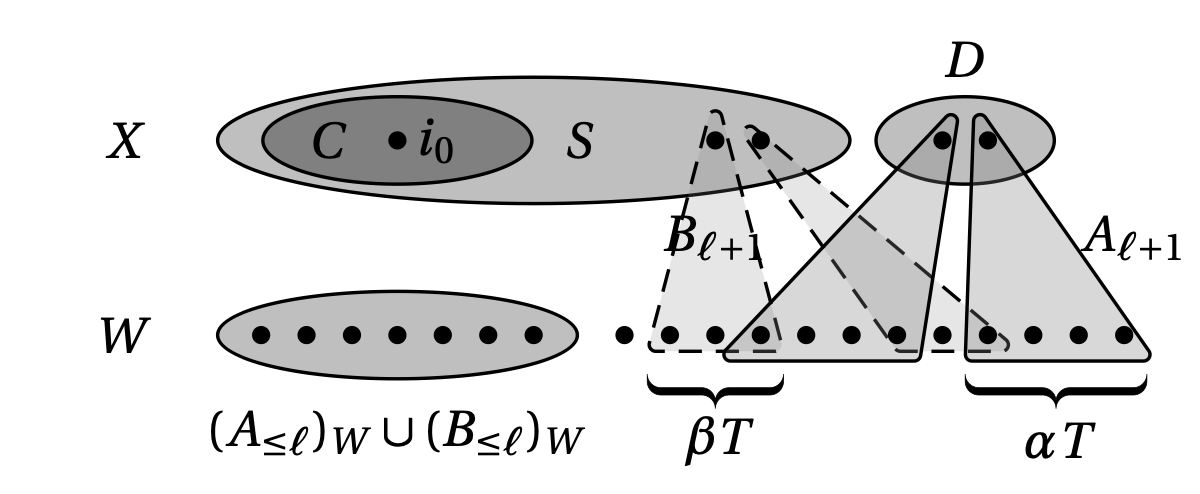
\includegraphics[width=10cm]{chapters/santaclaus/SC_fig2.png}
    \caption{Case 1 of the algorithm, 
    where a set $A_{\ell+1} \subseteq \pazocal{E}_{\alpha T}$ of hyperedges is found that intersects many new edges $
    B_{\ell+1} \subseteq (M \setminus B_{\leq \ell})$. In particular $|B_{\ell+1}| \geq \Omega_{\varepsilon}(|C|)$. 
    Note that $D$ might contain nodes from $C$.\label{fig:CaseIofTheAlgorithm}}
\end{center}
\end{figure}

\begin{figure}
    \begin{center}
        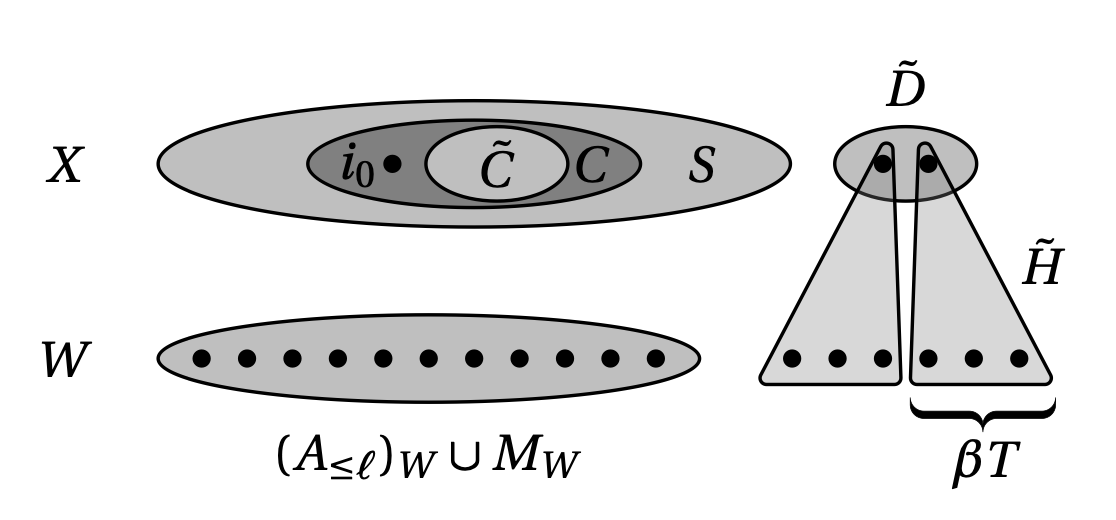
\includegraphics[width=10cm]{chapters/santaclaus/SC_fig3.png}
        \caption{Case 2 of the algorithm, 
        where $\tilde{H} \subseteq \pazocal{E}_{\beta T}$ of size $|\tilde{H}| \geq \Omega_{\varepsilon}(|C|)$ 
        is found so that $(i)$ $\tilde{H}$ is disjoint on the $W$-side to the matching $M$ and the adding edges in the augmenting tree, 
        $(ii)$ $\tilde{H}$ covers a set $\tilde{D}$ with $S \setminus \tilde{C} \cup \tilde{D} \in \pazocal{I}$, 
        and $(iii)$ $\tilde{C}$ is from one layer of the augmenting tree. 
        Here $\tilde{D}$ and $\tilde{C}$ do not have to be disjoint.\label{fig:CaseIIofTheAlgorithm}}
    \end{center}
    \end{figure}
% \begin{subfigure}{}
% \psset{xunit=0.7cm,yunit=0.5cm}
% \begin{pspicture}(-1,-2)(12,5)
% %\psset{linecolor=lightgray}
% %\psgrid[gridcolor=lightgray,subgridcolor=white](-2,-3)(12,5)
% \rput[c](0,3){$X$}
% \rput[c](0,0){$W$}
% %\psellipse(0,0)(1,1)
% \psellipse[linewidth=0.75pt,fillstyle=solid,fillcolor=lightgray](4.5,3)(3.5,1)\rput[c](5,3){$S$}% S
% \psellipse[linewidth=0.75pt,fillstyle=solid,fillcolor=gray](3,3)(1.5,0.7)\rput[c](2.25,3){$C$}% C
% \psellipse[linewidth=0.75pt,fillstyle=solid,fillcolor=lightgray](9.25,3)(1.0,0.7)\rput[c](9.25,4.25){$D$}% D
% \psellipse[linewidth=0.75pt,fillstyle=solid,fillcolor=lightgray](3,0)(2,0.7)\rput[c](3,-1.5){$(A_{\leq \ell})_W \cup (B_{\leq \ell})_W$}% A_W + B_
% % EDGES IN B_l+1
% %\pspolygon(6.5,3)(6,0)(7,0)
% \pspolygon[linearc=0.05,linewidth=0.75pt,linestyle=dashed,opacity=0.2,fillcolor=gray,fillstyle=solid](6.5,3.75)(5.75,-0.25)(7.25,-0.25)\rput[c](6.5,1.5){$B_{\ell+1}$}
% %\pspolygon(7.0,3)(8.5,0)(10,0)
% \pspolygon[linearc=0.05,linewidth=0.75pt,linestyle=dashed,opacity=0.2,fillcolor=gray,fillstyle=solid](6.5,3.7)(8.5,-0.25)(9.85,-0.25)
% % EDGES IN A_l+1
% %\pspolygon[linecolor=blue](9,3)(7,0)(8.5,0)
% \pspolygon[linearc=0.05,linewidth=0.75pt,linecolor=black,opacity=0.3,fillcolor=gray,fillstyle=solid](9.2,3.6)(6.5,-0.4)(8.75,-0.4)
% %\pspolygon[linecolor=blue](9.5,3)(9.5,0)(11,0)
% \pspolygon[linearc=0.05,linewidth=0.75pt,linecolor=black,opacity=0.3,fillcolor=gray,fillstyle=solid](9.35,3.6)(9.25,-0.4)(11.35,-0.4)\rput[l](10.5,1.5){$A_{\ell+1}$}
% % NODES IN X AND W
% \multido{\N=1.5+0.5}{7}{\cnode*(\N,0){2pt}{A}}
% \multido{\N=5.5+0.5}{12}{\cnode*(\N,0){2pt}{A}}
% \cnode*(3,3){2pt}{i0}\nput[labelsep=2pt]{0}{i0}{$i_0$}
% \cnode*(6.5,3){2pt}{B1}
% \cnode*(7.0,3){2pt}{B1}
% \cnode*(9.0,3){2pt}{A1}
% \cnode*(9.5,3){2pt}{A1}
% %\psbrace[rot=90,ref=1C,nodesepB=5pt](1,-1)(5,-1){$(A_{\leq \ell})_W \cup (B_{\leq \ell})_W$}
% \psbrace[rot=90,ref=1C,nodesepB=7pt,braceWidthInner=3pt,braceWidthOuter=3pt](5.75,-0.6)(7.25,-0.6){$\beta T$}
% \psbrace[rot=90,ref=1C,nodesepB=7pt,braceWidthInner=3pt,braceWidthOuter=3pt](9.25,-0.6)(11.25,-0.6){$\alpha T$}
% \end{pspicture}
% \caption{Case 1 of the algorithm, where a set $A_{\ell+1} \subseteq \pazocal{E}_{\alpha T}$ of hyperedges is found that intersects many new edges $B_{\ell+1} \subseteq (M \setminus B_{\leq \ell})$. In particular $|B_{\ell+1}| \geq \Omega_{\varepsilon}(|C|)$. Note that $D$ might contain nodes from $C$.\label{fig:CaseIofTheAlgorithm}}
% \end{subfigure}
% %\end{center}
% %\begin{center}
% \begin{subfigure}{}
% \psset{xunit=0.7cm,yunit=0.5cm}
% \begin{pspicture}(-1,-1.5)(12,5.5)
% %\psset{linecolor=lightgray}
% %\psgrid[gridcolor=lightgray,subgridcolor=white](-2,-3)(12,5)
% \rput[c](0,3){$X$}
% \rput[c](0,0){$W$}
% %\psellipse(0,0)(1,1)
% \psellipse[linewidth=0.75pt,fillstyle=solid,fillcolor=lightgray](4.5,3)(3.5,1)\rput[c](7.0,3){$S$}% S
% \psellipse[linewidth=0.75pt,fillstyle=solid,fillcolor=gray](4.5,3)(1.85,0.7)\rput[c](5.8,3){$C$}% C
% \psellipse[linewidth=0.75pt,fillstyle=solid,fillcolor=lightgray](4.75,3)(0.8,0.6)\rput[c](4.75,3){$\tilde{C}$}% \tilde{C}
% \psellipse[linewidth=0.75pt,fillstyle=solid,fillcolor=lightgray](9.25,3)(0.8,0.6)\rput[c](9.25,4.25){$\tilde{D}$}% D
% \psellipse[linewidth=0.75pt,fillstyle=solid,fillcolor=lightgray](4.0,0)(3,0.7)\rput[c](4,-1.5){$(A_{\leq \ell})_W \cup M_W$}% A_W + B_W
% % EDGES IN A_l+1)
% \pspolygon[linearc=0.05,linewidth=0.75pt,linecolor=black,opacity=0.3,fillcolor=gray,fillstyle=solid](9.1,3.6)(7.6,-0.4)(9.20,-0.4)
% \pspolygon[linearc=0.05,linewidth=0.75pt,linecolor=black,opacity=0.3,fillcolor=gray,fillstyle=solid](9.4,3.6)(9.30,-0.4)(10.90,-0.4)\rput[l](10.5,1.5){$\tilde{H}$}
% % NODES IN X AND W
% \multido{\N=1.5+0.5}{11}{\cnode*(\N,0){2pt}{A}}
% \multido{\N=8.00+0.50}{6}{\cnode*(\N,0){2pt}{A}}
% \cnode*(3.6,3){2pt}{i0}\nput[labelsep=1pt]{180}{i0}{$i_0$}
% \cnode*(9.0,3){2pt}{A1}
% \cnode*(9.5,3){2pt}{A2}
% %\psbrace[rot=90,ref=1C,nodesepB=5pt](1,-1)(5,-1){$(A_{\leq \ell})_W \cup (B_{\leq \ell})_W$
% \psbrace[rot=90,ref=1C,nodesepB=7pt,braceWidthInner=3pt,braceWidthOuter=3pt](9.30,-0.6)(10.90,-0.6){$\beta T$}
% \end{pspicture}
% \end{subfigure}
% \caption{Case 2 of the algorithm, where $\tilde{H} \subseteq \pazocal{E}_{\beta T}$ of size $|\tilde{H}| \geq \Omega_{\varepsilon}(|C|)$ is found so that $(i)$ $\tilde{H}$ is disjoint on the $W$-side to the matching $M$ and the adding edges in the augmenting tree, $(ii)$ $\tilde{H}$ covers a set $\tilde{D}$ with $S \setminus \tilde{C} \cup \tilde{D} \in \pazocal{I}$, and $(iii)$ $\tilde{C}$ is from one layer of the augmenting tree. Here $\tilde{D}$ and $\tilde{C}$ do not have to be disjoint.\label{fig:CaseIIofTheAlgorithm}}
% \end{center}
% \end{figure}


\subsection{Termination and runtime}



  As seen in Lemma~\ref{lem:ConstantSizeSwap}, 
\[
|X| \geq |B_{\leq \ell}|\geq \big(1+\frac{\varepsilon^2}{4} \big)^{\ell}|B_0|,
\]
and solving for $\ell$ shows $\frac{\log(|X|)}{\log \big(1+\frac{\varepsilon^2 }{4} \big)}  \geq \ell$.
Thus the total number of layers at any step in the algorithm is $O(\log|X|)$. 
Note after each collapse of the layers, the matching $M$ and possibly the independent set $S$ are updated. 
However, the fixed exposed node $i_0$ will remain in $S$ until the very last iteration in which the algorithm finds
an edge $e_1$ that augments the matching. 
Before we begin discussing the proof guaranteeing our algorithm terminates, we need a lemma to compare the number of blocking edges after a layer is collapsed to the number of blocking edges at the beginning of the iteration. 

\begin{lemma}\label{lem:ExtraSteps}
  Let $\tilde{\ell}$ be the index of the collapsed layer and let $B'$ be the updated blocking edges after a collapse step. Then,
  $|B'_{\leq \tilde{\ell}}| \leq |B_{\leq \tilde{\ell}}| \cdot (1- \frac{\varepsilon^2}{4} \cdot \gamma )$.
\end{lemma}
\begin{proof}
 Recall $B'_{\tilde{\ell}} = B_{\tilde{\ell}} \setminus F$ for $F$ the edges of $M$ covering $\tilde{C}$. Further, the blocking edges in layers indexed less than $\tilde{\ell}$ are not effected in the iteration. Hence
 \begin{eqnarray*}
  |B'_{\leq \tilde{\ell}}| &=& |B'_{\leq \tilde{\ell}-1}| + |B'_{ \tilde{\ell}}|=|B_{\leq \tilde{\ell}-1}| + |B'_{ \tilde{\ell}}| 
\end{eqnarray*}
From Lemmas~\ref{lem:GreedyMatchingExpansionLemma} and~\ref{lem:SizeOfOverlapOfNewEdgesWithM},
$|B_{\ell+1}| \geq \frac{\varepsilon^2}{4}|B_{\leq \ell}|$. Then examining the collapsed layer by itself, we see 
\begin{eqnarray*}
  |B'_{ \tilde{\ell}}| &=& |B_{ \tilde{\ell}}|-|F| \leq |B_{ \tilde{\ell}}| -   \frac{\varepsilon^2}{4} \cdot \gamma |B_{ \leq \tilde{\ell}}|.
\end{eqnarray*}
Substituting back into $|B'_{\leq \tilde{\ell}}|$, we find that
\begin{eqnarray*} 
  |B'_{\leq \tilde{\ell}}| &\leq& |B_{\leq \tilde{\ell}-1}| + |B_{ \tilde{\ell}}| -  \frac{\varepsilon^2}{4} \cdot \gamma |B_{ \leq \tilde{\ell}}| \\
  &=& |B_{\leq \tilde{\ell}}| - \frac{\varepsilon^2}{4} \cdot \gamma |B_{ \leq \tilde{\ell}}| =|B_{ \leq \tilde{\ell}}| 
  \cdot \big (1-\frac{\varepsilon^2}{4} \cdot \gamma \big).
\end{eqnarray*}
\end{proof}

To prove the algorithm terminates in polynomial time, we consider a signature vector $s = (s_0,s_1,\ldots, s_{\ell}, \infty)$, 
where $s_j = \lfloor \log_{c}|B_{\leq j}| \rfloor $ for $c = \frac{1}{1-\frac{\varepsilon^2 }{4}\cdot \gamma}$. 
The signature vector and proof that the algorithm terminates is inspired by \cite{AlgoForSantaClaus-AnnamalaiKalaitzisSvenssonSODA15}, 
but it is subtly different. 


\begin{lemma}\label{lem:LexOrderDecreases}
The signature vector decreases lexicographically after each iterative loop in the algorithm. 
\end{lemma}
\begin{proof}
Let $s = (s_0,\ldots,s_{\ell},\infty)$ be a signature vector at the beginning of a step in the algorithm, and let $s'$ be the result of $s$ through one iteration of the algorithm. For $\ell+1$ denoting the newest built layer in the algorithm, if the newest set of hyperedges found intersects at least $\frac{\varepsilon^2}{4}|C|$ many edges of $M$, then another layer in the augmenting tree is built and no layer is collapsed. Then $s' = (s_0,\ldots,s_{\ell},s_{\ell+1},\infty)$ is lexicographically smaller than $s$.

Otherwise, layer $0 \leq \tilde{\ell} \leq \ell$ is collapsed. All finite coordinates above $s_{\tilde{\ell}}$ are deleted from the signature vector, and all coordinates before $s_{\tilde{\ell}}$ are unaffected. So it suffices to check that $s'_{\tilde{\ell}} < s_{\tilde{\ell}}$. Again, let $B'$ be the updated blocking edges after a collapse step. As $B_{\tilde{\ell}}$ is the only set of blocking edges in $B_{\leq \tilde{\ell}}$ affected by the collapse, by Lemma~\ref{lem:ExtraSteps} one has $|B'_{\leq \tilde{\ell}}| \leq |B_{\leq \tilde{\ell}}|(1-\frac{\varepsilon^2}{4} \cdot \gamma )$. Taking a $\log$ we compare the coordinates
\[
s'_{\tilde{\ell}} = \left \lfloor \log_c \left ( \left |B'_{\leq \tilde{\ell}} \right | \right ) \right \rfloor \leq \left \lfloor \log_c \left ( \left |B_{\leq \tilde{\ell}} \right | \left (1- \frac{\varepsilon^2}{4} \cdot \gamma \right ) \right) \right \rfloor= 
\left \lfloor \log_c \left ( \left | B_{\leq \tilde{\ell}} \right | \right ) \right \rfloor -1 = s_{\tilde{\ell}}-1.
\]
\end{proof}
Choose the infinite coordinate to be some integer larger than $\log |X|$.  Since for every layer $\ell$, we have $|B_{\leq \ell}| \leq |X|$, then every coordinate of the signature vector is upper bounded by $U = O(\log |X|)$. Recall the number of layers, and thus the number of coordinates in the signature vector, is also upper bounded by $U$. Together, these imply that the sum of the coordinates of the signature vector is at most $U^2$. 

As the signature vector has non-decreasing order, each signature vector corresponds to a partition of an integer $z \leq U^2$. On the other hand, every partition of some $z \leq U^2$ has a corresponding signature vector. Thus we apply a result of Hardy and Ramanujan to find the total number of signature vectors is $\sum_{k \leq U^2} e^{O(\sqrt{k})} = |X|^{O(1)}$. Since each iteration of the algorithm can be done in polynomial time and the signature vector decreases lexicographically after each iteration, the algorithm terminates after a total time of $n^{\Theta_{\varepsilon}(1)}$. 

%\textbf{Theorem 5 to Thorem 2}- $|W|$ is different in the unit case than in the general case. To ensure this doesn't effect runtime, do we need to be more careful in splitting items than scaling everything so the smallest $p_j$ is 1, then breaking up the rest of the jobs into unit sizes? In particular, there's some assumption that $\{p_j\} \in \mathbb{Z}$ here. 



\section{Application to Santa Claus\label{sec:SantaClausApplication}}

In this section, we show a polynomial time $(4+\varepsilon)$-approximation algorithm
for the Santa Claus problem. Recall that 
for a given set of children $M$, and a set of presents $J$, the Santa Claus problem asks how Santa should distribute presents to children in order to maximize the minimum happiness of any child\footnote{We assume Santa to be an equitable man-- not one influenced by bribery, social status, etc.}.
Here, present $j$ is only wanted by some subset of children that we denote by $A_j \subseteq M$, and present $j$ has value $p_{j}$ to child $i \in A_j$. The happiness of child $i$ is the sum of all $p_{j}$ for presents $j$ assigned to child $i$. 
%We consider a restricted version of this problem where $p_{ij} \in\{0,p_j\}$, so $p_{ij}=0$ for all children $i$ such that $j \not \in A_i$ and otherwise children who want present $j$ all value it equally. 
We assume w.l.o.g. to know the integral objective function value $T$ of the optimum solution,
otherwise $T$ can be found by binary search.

We partition gifts into two sets: \emph{large} gifts $J_L := \{ j \in J \mid p_j > \delta_2 T\}$
and \emph{small} gifts $J_S := \{ j \in J \mid p_j \leq \delta_1 T\}$,
for parameters $0 < \delta_1 \leq \delta_2 < 1$ such that
% For fixed parameters $1 \geq \delta_2 \geq 1/4 > \delta_1 \geq 0$, where 
all gifts have values in $[0,\delta_1  T] \cup (\delta_2  T,T]$. 
Let $P(T,\delta_1,\delta_2)$ be the set of vectors $z \in \mathbb{R}_{\geq 0}^{J \times M}$ satisfying
\begin{eqnarray*}\label{eq:CompactLPforSC}
 \sum\limits_{j \in J_S: i \in A_j} p_j z_{ij} &\geq& T \cdot \Big( 1-\sum_{j \in J_L: i \in A_j} z_{ij}\Big)  \qquad \forall i \in M \\
  \sum\limits_{i \in A_j}z_{ij} &\leq& 1 \hspace{4.0cm} \forall j \in J \\
  z_{ij} &\leq& 1-\sum_{j' \in J_L: i \in A_{j'}} z_{ij'} \hspace{1.5cm} \forall j \in J_S \; \forall i \in A_j
\end{eqnarray*}

% \rem{S, Y: Should we be dropping unnecesary large jobs, or defining the basis of the matroid to be the machines forming the \textit{largest} matchings on $L$, not those forming $L$-perfect matchings}
If $n = |J| + |M|$, then this LP has $O(n^2)$ many variables and $O(n^2)$
many constraints. To see that this is indeed a relaxation, take any feasible assignment $\sigma : J \to M$ with $\sum_{j \in \sigma^{-1}(i)} p_j \geq T$ for all $i \in M$. 
Now let $\sigma : J \to M \cup \{ \emptyset \}$ be a modified 
assignment where we set $\sigma(j) = \emptyset$ for gifts that we decide to drop. For each child $i \in M$ that receives at least one large gift 
we drop all small gifts and all but one large gift. 
Then a feasible solution $z \in P(T,\delta_1,\delta_2)$ is obtained by letting  
\[ 
  z_{ij} := \begin{cases} 
 1 & \textrm{if }\sigma(j) = i \\
%1 & \textrm{if }\sigma(j) = i\textrm{ and }p_j \geq \delta \dot T  \\
%1 & \textrm{if }\sigma(j) = i\textrm{ and }p_j < \delta T\textrm{ and }\not\exists j'\textrm{ with } (\sigma(j')=i\textrm{ and }p_j' \geq \delta T)\\
0 & \textrm{otherwise}.
\end{cases}
\]


% The problem gives rise to the following linear program:


% \[\max \quad  T \]
% \[\sum\limits_{j \in J} p_{ij}x_{ij} \geq T \qquad \forall i \in M \]
% \[ \sum\limits_{i \in M} x_{ij} = 1 \qquad \forall j \in J \]
% \[ 0 \leq x_{ij} \leq 1 \qquad \forall i \in M, \forall j \in J,\]
% where $x_{ij}$ is the indicator variable for giving gift $j$ to child $i$. The first constraint ensures each child receives enough ``happiness'' and the second constraint ensures all gifts are assigned. 
% % This formulation has an unbounded integrality gap, as can be seen by considering the case when there are 2 machines which only admit jobs $j_1$ and $j_2$, where $p_{j_1} = 1$ and $p_{j_2}=T$ for large $T$. 


We will show that given a feasible solution $z \in P(T, \delta_1,\delta_2)$, there exists a feasible solution $(x^*,y^*)$ to $Q(T)$. To do this, we will exploit two underlying matroids in the Santa Claus problem, allowing us to apply Theorem~\ref{thm:MainMatroidAlgorithm}. Let 
\[
  \pazocal{I} = \left\{M_L \subseteq M |\; \exists \text{ left-perfect matching between } M_L\textrm{ and }J_L\textrm{ using edges }(i,j): i \in A_j\right\}, 
\]
be a family of independent sets. Then  $\pazocal{M} = (M,\pazocal{I})$ constitutes a \emph{matchable set matroid}.
% $\pazocal{M}$ obviously satisfies nonemptyness and monotonicity. For a proof that it satisfies the swapping condition, see section 10.3 in Schrijver's notes. 
%The bases of this matroid are 
%\[
%  \pazocal{B}(\pazocal{M}) = \{ M_L \subset M  | \quad \exists L \text{ perfect matching covering }M_L\}.
%\]
We denote the \emph{co-matroid} of $\pazocal{M}$ by $\pazocal{M}^* = (M, \pazocal{I}^*)$. Recall that the  independent sets 
of the co-matroid are given by
\[
  \pazocal{I}^* = \left\{M_S \subseteq M | \; \exists  M_L \in \pazocal{B}(\pazocal{M}):  M_S \cap M_L = \emptyset \right\}.
\]
% \[ \pazocal{B}(\pazocal{M}^*) = \{M_S \subset M | \quad M_S = M \setminus M_L \quad M_L \in \pazocal{B}(\pazocal{M}) \}
%\]


We can define a vector $x \in \setR^M$ with 
$ 
x_i = \sum_{j \in J_L: i \in A_j} z_{ij}
$
that lies in the matroid polytope of $\pazocal{M}$. This fact follows easily from the integrality of the fractional matching polytope in bipartite graphs. It is instructive to think of $x_i$ as the decision variable telling whether child $i \in M$ should receive a large present.

%For any $U \subseteq M$, $z(U)$ is the load between $U$ and large jobs admissable on $U$. As no node in this subgraph gives or receives load more than 1, $z(U)$ is upper bounded by the size of the minimum vertex cover, since otherwise some node in the minimum vertex cover would give or receive load more than 1. By K{\H o}nig's theorem, $z(U) \leq \textrm{rank}(U)$ with respect to the matchable set matroid.
Unfortunately, $x$ does not have to lie in the base polytope --- in fact the sum $\sum_{i \in M} x_i$ might not even be integral. 
%Given the existence of this vector $z$, using the following lemma, we find $z'$ in the base polytope of $\pazocal{M}$ where every machine is just as well covered with large jobs as in $z$.
However, there always exists a vector $x'$ in the base polytope that covers
every child just as well with large presents as $x$ does. 
%Recall the following fact from matroid theory: 
This observation can be stated for general matroids: 
\begin{lemma}\label{lem: RoundToBasePolytope}
Let $\pazocal{M} = (X,\pazocal{I})$ be any matroid and let $x$ be a point in its matroid polytope. Then in polynomial time one can find a point $x'$ in the base polytope so that $x' \geq x$ coordinate-wise. 
\end{lemma}
In fact the algorithm behind this claim is rather trivial: as long as $x \in P_{\pazocal{M}}$ is not in the base polytope, there is always a coordinate $i$ and a $\mu>0$ so that $x+\mu e_i \in P_{\pazocal{M}}$.

% \rem{Y: I changed $z+\delta e_i$ into $x+\delta e_i$, which should be just a typo.}

With the new vector $x' \in P_{\pazocal{B}(\pazocal{M})}$ at hand, we can redefine the $z$-assignments by letting
\[ 
  z_{ij}' = 
\begin{cases}
z_{ij} & \qquad x_i = 1\\ 
\frac{1-x_i'}{1-x_i} z_{ij} & \qquad x_i \neq 1.
\end{cases} 
\]
for $j \in J_S$; the new values $z_{ij}'$ for $j \in J_L$ can be obtained from the fractional matching
that corresponds to $x_i'$. Note that $0 \leq z_{ij}' \leq z_{ij}$ for $j \in J_S$. The reader should be convinced that
still $z' \in P(T,\delta_1,\delta_2)$, just that the corresponding vector $x'$ now lies in $P_{\pazocal{B}(\pazocal{M})}$\footnote{There is an alternative proof without the need to replace $x$ by $x'$. Add the constraint $\sum_{j \in J_L, i \in A_j} z_{ij} = \textrm{rank}(\pazocal{M})$
to $P(T,\delta_1, \delta_2)$. There is always a feasible integral solution satisfying this constraint. Then for any fractional solution $z \in P(T,\delta_1,\delta_2)$, the corresponding vector $x$ will immediately lie in the base polytope.}.

% \rem{Y: For the footnote, I am wondering if this change will make binary search difficult, since we need to define a matroid for each T.}

%Note that $y^*_{ij}$ is smaller than $y_{ij}$, as more machines are covered with large jobs. 
%With the overall goal of finding some pair feasible to $Q(T)$, we next observe that $x = 1-z'$ is in the base polytope of the comatroid $\pazocal{M}^*$.
It is well known in matroid theory that  
the complementary vector $x^* := \mathbb{1} - x'$ lies in $P_{\pazocal{B}(\pazocal{M}^*)}$. 
Again, it is instructive to think of $x^*_i$ as the decision variable whether 
child $i$ has to be satisfied with small gifts.
Finally, the assignments $y^*$ are simply the restriction of $z'$ on the 
coordinates $(i,j) \in M \times J_S$.
The obtained pair $(x^*,y^*)$ lies in $Q(T)$, where the matroid in the definition 
of $Q(T)$ is $\pazocal{M}^*$.
%\begin{lemma}\label{lem: ComplementBase}
%  Let $\pazocal{M} = (X,\pazocal{I})$ be any matroid and let $z$ be a point in the base polytope. Then one has that $1-z$ is in the base polytope of the comatroid of $\pazocal{M}$, $\pazocal{M}^*$.
%\end{lemma}

%The $x$ defined above is that which will be a part of the solution to $Q(T)$, and it remains to scale $y$ to find $y^*$. Restricting $y^*$ to the coordinates of $Q(T)$ and then substituting in $(x,y^*)$ for $Q(T)$, one sees it is a feasible solution.



% Let $G_{(T,\delta)} = (M \cup S, E_S)$ be the bipartite graph with $E_S$ the set of edges between children and small gifts, and let $N(i)$ denote the neighborhood of node $i$ in $E_S$ (to avoid $\delta$s with different meanings here).
% Now, we're able to rewrite $Q(T)$ as a linear program $P(T,\delta)$:
 

% \[\max \quad  T \]
% \[x \in P_{\pazocal{B}(\pazocal{M}^*_{(T,\delta)})}\]
% \[\sum\limits_{j \in N(i)} p_j y_{ij} \geq T \cdot x_i \qquad \forall i \in X\]
% \[ y(N(j)) \leq 1 \qquad \forall j \in S\]
% \[  y_{ij} \leq x_i \qquad \forall (i,j) \in E_S\]
% \[(x,y) \in \mathbb{R}_{\geq 0}^{M} \times \mathbb{R}_{\geq 0}^{E_S}\]


As $Q(T) \neq \emptyset$, we can apply Theorem~\ref{thm:MainMatroidAlgorithm} 
which results in a subset $M_S \in \pazocal{B}(\pazocal{M}^*) $
 of the children and an assignment $\sigma : J_S \to M_S$, 
where each child in $M_S$ receives happiness at least 
$ \big(\frac13 - \frac{\delta_1}{3} - \varepsilon \big) \cdot T$ from the assignment of small gifts.
Implicitly due to the choice of the matroid $\pazocal{M}^*$, 
we know that the remaining children $M \setminus M_S = M_L$ can all receive one large gift
and this assignment can be computed in polynomial time using a matching algorithm. 
Overall, each child receives either one large present of value
at least $\delta_2 \cdot T$ or small presents of total value at least $(\frac{1}{3} - \frac{\delta_1}{3}-\varepsilon ) \cdot T$. 
Therefore each child receives value at least
\begin{equation}\label{eq: balanceSC}
  \min\Big\{ \Big(\frac{1}{3}-\frac{\delta_1}{3}-\varepsilon\Big) \cdot T, \delta_2 \cdot T \Big\} \geq \Big(\frac{1}{4}-\varepsilon\Big) \cdot T
\end{equation}
for a choice of $\delta_2 = \delta_1=\frac{1}{4}$. 
In some instances of Santa Claus, we can do better. 
Set $\delta_1$ so that $\delta_1 \cdot T$ is the largest gift value
that is at most $\frac14 T$, and set $\delta_2$ so that $\delta_2 \cdot T$ 
is the smallest gift value that is at $\frac14 T$.
Then the algorithm guarantees that each child receives value at least 
as in the left hand side of Equation~\ref{eq: balanceSC}. 
When $\delta_1$ and $\delta_2$ are bounded away from $1/4$,
then the approximation improves. 
For example, when $\delta_2 \geq 1/3$ and $\delta_1 T$ is close to 0,
such as in the case where all gifts have value either $T$ or 1,
we approach a $(3+\varepsilon)$-approximation.

\section{Conclusion}
In this work, we introduced Matroid Max-Min Fair Allocation. 
for this problem, we construct a new, compact LP to model it, 
and we prove a $(3+\epsilon)$-approximation, modulo an additive term of $\frac13$ of the most valuable item's value $\frac13 \max_{w in W} p_w$.
Our algorithm is a local search based on Haxell's augmenting tree argument.
Overall, we can use our result on Matroid Max-Min Fair Allocation as a blackbox to obtain a $(4+\epsilon)$-approximation for Santa Claus.


One obvious, immediate open question is to resolve the gap between the lower bound of 2 and the upper bound of 4 for approximation Santa Claus.
We do not know the integrality gap for our LP, so it is unclear whether the LP can be used to obtain approximations better than 4. 
More broadly, this problem of Matroid Max-Min Fair Allocation might be useful to study other scheduling problems. 





%, which is in $\pazocal{B}(\pazocal{M})$ by definition of $\pazocal{B}(\pazocal{M}^*)$. In polynomial time, we can find a matching between $M_L$ and $L$. Thus we have an assignment that assigns each child either one large gift, and thus happiness at least $\delta \cdot T$, or enough small gifts to have happiness at least $(\frac13 - \varepsilon - \delta) \cdot T$. A choice of $\delta \approx \frac16$ maximizes all children's happiness.




%In particular this sets $y_{ij} = 0$ for small jobs that are unnecessary because $i$ already receives a large job.

